\documentclass[a4paper,11pt,fleqn]{article}%fleqn pour aligner les equations à gauche
\usepackage{../../Styles/Cours}

\newcommand{\chnum}{Chapitre 14}
\newcommand{\chtitle}{Vitesse des ondes sonores}
\newcommand{\dtype}{TP}

\begin{document}
	\maketitle
	
Lorsque le professeur d'adresse ax élèves depuis le bureau les élèves du premier rang  sont souvent les plus réactifs, alors que ceux du fond prennent plus longtemps à réagir et se mettre au travail.\\
Est ce qu'il y a un réel décalage temporel entre les instructions reçues par les élèves du premier et du dernier rang d'une classe ?
\vspace{1em}

\noindent\begin{minipage}[t]{.49\linewidth}
	\begin{documentboxenv}{Les ultrasons}
	L'oreille humaine ne perçoit que les sons dont la fréquence est comprise entre \SI{20}{\hertz} et \SI{20}{\kilo\hertz}. Au-delà de \SI{20}{\kilo\hertz}, il s'agit d'ultrasons. Les ultrasons se déplacent à la même vitesse que les sons audibles.
	\begin{center}
		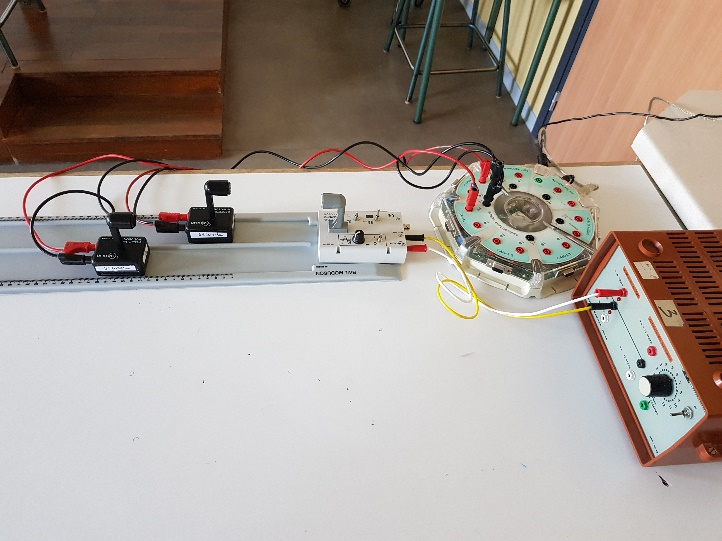
\includegraphics[scale=.35]{Ressources/2GT_C7_AE1_Fig3.png}
	\end{center}
	\end{documentboxenv}
\end{minipage}\hspace{.02\linewidth}
\begin{minipage}[t]{.49\linewidth}
	\begin{documentboxenv}{Réglage du matériel}
		\begin{itemize}[leftmargin=5pt]
		\item L'émetteur à ultrasons $E$ est alimenté avec une tension continue de \SI{15}{V}.
		\item Le récepteur à ultrasons transforme le signal perçu en signal électrique de même fréquence. On visualise les variations de ce signal électrique sur l'ordinateur.
		\item Sélectionner le mode continu sur l'émetteur $E$
		\item Pour pouvoir enregistrer les signaux reçus, relier le récepteur 1 en $EA0$, le récepteur 2 en $EA1$ (ne pas oublier de relier les masses en noir à celle de la carte d'acquisition)
		\item Aligner l'émetteur et les deux récepteurs le long d'un rail gradué.
	\end{itemize}
	\end{documentboxenv}
\end{minipage}

\vspace{1em}
\noindent\begin{documentboxenv}{Réglage du logiciel LatisPro}
	\begin{minipage}{.65\linewidth}
	\begin{itemize}[leftmargin=5pt]
		\item Ouvrir le logiciel LatisPro
		\item Cliquer sur les voies $EA0$ et $EA1$ pour les activer
		\item Changer le style de courbe. Pour cela, faire un clic-droit sur la légende $EA1$ et cliquer sur "Propriétés" puis "Style" et choisir "Trait". Valider "Ok". N'oublier pas de faire la même chose avec $EA0$.
	\end{itemize}
\end{minipage}\hspace{1em}
\begin{minipage}{.3\linewidth}
	\centering 
	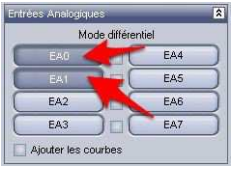
\includegraphics[width=\linewidth]{Ressources/2GT_C7_AE1_Fig1.png}\\
	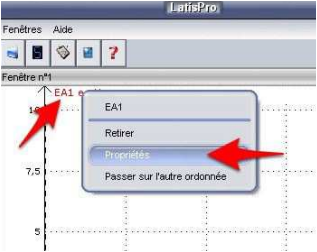
\includegraphics[width=\linewidth]{Ressources/2GT_C7_AE2_Fig1.png}
\end{minipage}
\end{documentboxenv}

\section*{Partie A : Période et fréquence de l'onde ultrasonore}

	\begin{protocole}
	\begin{itemize*}
		\item Sélectionner le mode continu sur l'émetteur $E$
		\item À gauche, sous "Acquisition", changer le nombre de points à mémoriser : taper 250 puis appuyer sur la touche "Entré". 
		\item Changer ensuite la durée totale : taper \SI{100}{\micro\second}, puis appuyer sur la touche "Entré".
		\item Sélectionner le mode permanent.
		\item Appuyer sur "déclenchement" et sélectionner $EA0$
		\item Lancer l'acquisition (F10)
		\item Pendant l'acquisition, faire un clic droit sur la zone graphique et cliquer sur "calibrage"
	\end{itemize*}
\end{protocole}

\begin{enumerate}
	\item Le signal reçu varie-t-il en fonction de la position du récepteur ? Justifier.
	\item Appuyer sur la touche "échap" pour arrêter l'acquisition. L'onde ultrasonore est dite "périodique". Expliquer ce terme et mesurer le temps caractéristique de ce phénomène périodique.\\
	Pour cela : faire un clic droit sur le graphique et choisir "Réticule". À l'aide du réticule, il sera plus facile de trouver $\Delta t$.
	\item Pour calculer la fréquence d'un signal périodique, on calcule l'inverse du temps caractéristique mesuré en question 2.\\
	Calculer la fréquence de l'onde observée.\\
	Vérifier qu'il s'agit bien d'ultrasons.
\end{enumerate}

\section*{Partie B : Célérité de l'onde ultrasonore}
\noindent \fbox{\begin{minipage}{.95\linewidth}
		\textbf{Manipulation à faire :}
	\begin{itemize*}
		\item Sélectionner le mode salves de l'émetteur $E$.
		\item À gauche, sous "Acquisition", changer le nombre de points à mémoriser : taper 500 puis appuyer sur la ouche "Entrer".\\
		Changer la durée totale : taper 20 ms, puis appuyer sur la touche "Entrer".\\
		Sélectionner le mode permanent et sans déclenchement.\\
		Appuyer sur "déclenchement", et sélectionner "aucun".
		\item Lancer l'acquisition (F10 ou cliquer sur le bouton triangulaire) puis, pendant l'acquisition, faire un clic droit dans la zone graphique et cliquer sur "calibrage".
		\item Appuyer sur la touche "échap" pour arrêter l'acquisition.
	\end{itemize*}
\end{minipage}}

\begin{enumerate}[resume]
	\item Comment varie le graphique obtenu lorsque la distance entre les deux récepteurs varie ? Pourquoi ?
	\item On nomme $\Delta t$ la différence de temps de réception entre les deux récepteurs.\\ Quelle est la relation donnant la vitesse des ultrasons en fonction de la distance entre les deux récepteurs et $\Delta t$ ?
	\item Faire varier la distance entre les deux récepteurs. Mesurer $\Delta t$ entre les pics maximaux des deux récepteurs et remplir le tableau ci-dessous :
\end{enumerate}
\begin{center}
	\renewcommand{\arraystretch}{2.2}
\begin{tabular}{|>{\centering}m{2cm}|>{\centering}m{2cm}|>{\centering}m{2cm}|>{\centering}m{2cm}|>{\centering}m{2cm}|>{\centering}m{2cm}|>{\centering\arraybackslash}m{2cm}|}
	\hline
	\rowcolor{gray!30} $d$ (m)&0,05&0,10&0,15&0,20&0,25&0,30\\
	\hline
	$\Delta t$& & & & & &\\
	\hline
	$v$ (\unit{\meter\per\second})& & & & & &\\
	\hline
\end{tabular}
\end{center}

\begin{enumerate}[resume]
	\item Calculer la vitesse moyenne
	\item Combien de temps met les signaux émis par le professeur au tableau pour parvenir aux oreilles des élèves du dernier rang de la classe ?
	\item De quels facteurs dépendent la vitesse des ultrasons ?
\end{enumerate}
\end{document}